\section{Durchschnittsgesicht und Differenzgesichter} \label{sec:facespace}
\begin{tcolorbox}
	\centerline{\textbf{Lernziele Kapitel~\ref{sec:facespace}}}
	\begin{enumerate}[leftmargin=*,label=\thesection.\arabic*]
		\item \label{item:meandiff_simple} Die Lernenden verstehen den Durchschnitt einer Familie von Vektoren sowie die Translation von Vektoren geometrisch.\\
		(Aufgabe~\ref{aufg:meandiff_simple})
		\item \label{item:meanface} Die Lernenden können die Addition von Vektoren und deren Multiplikation mit einem Skalar in Python ausführen.\\
		(Aufgabe~\ref{aufg:meanface})
		\item \label{item:hmmc} Die Lernenden können die Begriffe Durchschnittsgesicht und Differenzgesicht erklären.\\
		(Aufgabe~\ref{aufg:hmmc})
	\end{enumerate}
\end{tcolorbox}
Seien nun $M,N\in\mathbb N$ fix.
Wir haben im letzten Kapitel gesehen, wie man schwarz-weiss Bilder der Auflösung $M\times N$ als Vektoren in $\mathbb R^{M\cdot N}$ verstehen kann.
Die Bilder müssen dafür nicht unbedingt ein Gesicht zeigen.
Die Pixel können sogar völlig zufällige Graustufen aufweisen, so dass auf dem Bild nichts sinnvolles zu erkennen ist.
Dies führt uns zu folgender Beobachtung:
Nur die wenigsten Vektoren in $\mathbb R^{M\cdot N}$ entsprechen einem Gesicht.
Wir wollen uns näher mit dieser Beobachtung befassen.

Sei $K\in\mathbb N$ die Anzahl aller Bilder von allen Personen unserer Datenbank.
Jedes Bild soll dabei die Auflösung $M\times N$ haben.
Wir betrachten alle Bilder der Datenbank als Vektoren $\vec b_1,\ldots,\vec b_K\in\mathbb R^{M\cdot N}$.
Diese Darstellung erlaubt uns, das \textit{Durchschnittsgesicht}, wir nennen es $\vec m\in\mathbb R^{M\cdot N}$, zu definieren
\begin{equation*}
	\vec m=\frac{1}{K}\left(\vec b_1+\ldots+\vec b_K\right).
\end{equation*}
Um diesen Durchschnitt von Vektoren geometrisch besser zu verstehen, schauen wir das im $\mathbb R^2$ an.
\begin{aufgabe} \label{aufg:meandiff_simple}
	Betrachten Sie die folgenden drei Vektoren
	\begin{equation*}
		\vec{b}_1=
		\begin{pmatrix}
			-4 \\
			-5
		\end{pmatrix},\quad
		\vec{b}_2=
		\begin{pmatrix}
			9 \\
			-5
		\end{pmatrix},\quad
		\vec{b}_3=
		\begin{pmatrix}
			1 \\
			7
		\end{pmatrix}.
	\end{equation*}
	\begin{enumerate}[label=(\alph*)]
		\item Berechnen Sie den Durchschnitt $\vec{m}$ der Vektoren $\vec{b}_1,\vec{b}_1,\vec{b}_1$.
		\item Berechnen Sie die um $-\vec{m}$ verschobenen Vektoren
		\begin{equation*}
			\vec{a}_1=\vec{b}_1-\vec{m},\quad
			\vec{a}_2=\vec{b}_2-\vec{m},\quad
			\vec{a}_3=\vec{b}_3-\vec{m}.
		\end{equation*}
		\item Zeichnen Sie alle Vektoren $\vec{a}_1,\vec{a}_2,\vec{a}_3$ und $\vec{b}_1,\vec{b}_2,\vec{b}_3$, sowie $\vec{m}$ in ein Koordinatensystem.
	\end{enumerate}
\end{aufgabe}
\begin{losung*}
	\phantom{text}
	\begin{enumerate}[label=(\alph*)]
		\item Wie im skalaren Fall ist der Durchschnitt definiert als die Summe geteilt durch dir Anzahl der Summanden, also
		\begin{equation*}
			\vec{m}=\frac{1}{3}\left(\vec{b}_1+\vec{b}_2+\vec{b}_3\right)
			=\frac{1}{3}\left(
			\begin{pmatrix}
				-4 \\
				-5
			\end{pmatrix}+
			\begin{pmatrix}
				9 \\
				-5
			\end{pmatrix}+
			\begin{pmatrix}
				1 \\
				7
			\end{pmatrix}
			\right)
			=
			\begin{pmatrix}
				2 \\
				-1
			\end{pmatrix}.
		\end{equation*}
		\item Für die um $-\vec{m}$ verschobenen Vektoren erhalten wir folglich
		\begin{equation*}
			\vec{a}_1=
			\begin{pmatrix}
				-6 \\
				-4
			\end{pmatrix},\quad
			\vec{a}_2=
			\begin{pmatrix}
				7 \\
				-4
			\end{pmatrix},\quad
			\vec{a}_3=
			\begin{pmatrix}
				-1 \\
				8
			\end{pmatrix}.
		\end{equation*}
		\item Die Skizze ist in Abbildung~\ref{fig:meanddiff_simple} dargestellt.
		\begin{figure}[ht]
			\centering
			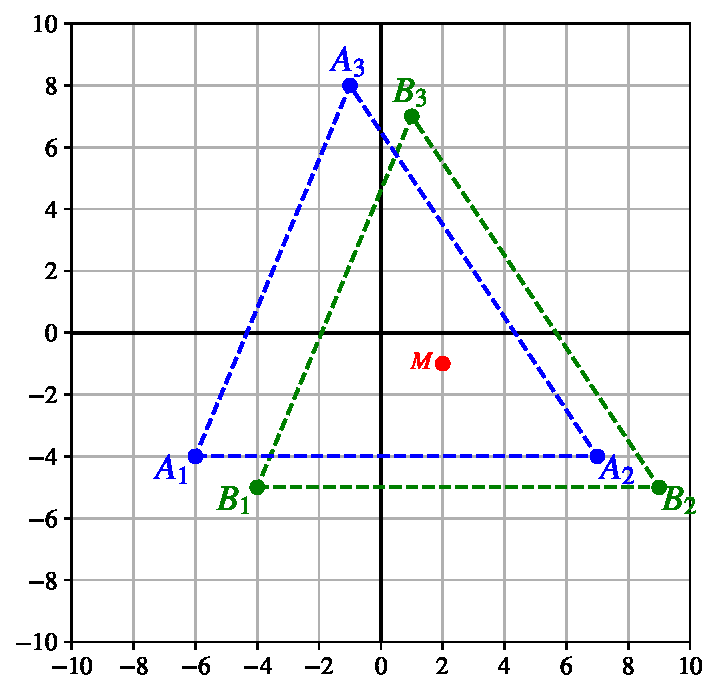
\includegraphics[width=0.5\textwidth]{images/facespace/meandiff_simple}
			\caption{Durchschnitt $\vec{m}$ der Vektoren $\vec{b}_1,\vec{b}_2,\vec{b}_3$ sowie deren Translationen $\vec{a}_1,\vec{a}_2,\vec{a}_3$ um $-\vec{m}$.}
			\label{fig:meanddiff_simple}
		\end{figure}
	\end{enumerate}
\end{losung*}
Das Durchschnittsgesicht lässt sich wieder als Bild ausgeben.
Aber wie sieht so ein Durchschnittsgesicht aus?
Das werden wir in folgender Übung herausfinden.
\begin{aufgabe} \label{aufg:meanface}
	Ergänzen Sie im File \texttt{eigenfaces.py} die Funktion \texttt{meanface(b\_list)}.
	Dabei ist \texttt{b\_list} die Liste der Länge $K$ der Vektoren $\vec b_1,\ldots,\vec b_K$.
	Der Rückgabewert soll das Durchschnittsgesicht $\vec m$ sein.
	Sie können die ihre Lösung überprüfen indem Sie das Skript \texttt{meanface\_test.py} laufen lassen.
	\textit{Hinweis:} Die Python Funktionen \texttt{len(...) und sum(...)} können nützlich sein.
\end{aufgabe}
\begin{losung*}
	Hier ist eine mögliche Lösung und das davon mit \texttt{meanface\_test.py} generierte Durchschnittsgesicht.\\[0.5cm]
	\begin{minipage}{0.45\textwidth}
\begin{lstlisting}[style=python]
def meanface(b_list):
	K = len(b_list)
	return sum(b_list) / K
\end{lstlisting}
	\end{minipage}\hfill
	\begin{minipage}{0.3\textwidth}\vspace{-1cm}
		\centering\hfill Durchschnittsgesicht:
	\end{minipage}
	\begin{minipage}{0.2\textwidth}\vspace{-1cm}
		\centering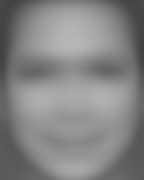
\includegraphics[width=0.6\textwidth]{images/facespace/meanface}
	\end{minipage}
\end{losung*}
Nachdem wir nun das Durchschnittsgesicht gebildet haben, berechnen wir nun die \textit{Differenzgesichter} $\vec a_1,\ldots,\vec a_K$.
Diese sind definiert als
\begin{equation*}
	\vec a_k=\vec b_k-\vec m,\quad k\in\left\{1,\ldots,K\right\}.
\end{equation*}
Die eben eingeführten Begriffe sind links in Abbildung~\ref{fig:meandiff} stark vereinfacht visualisiert.
\begin{figure}[ht]
	\centering
	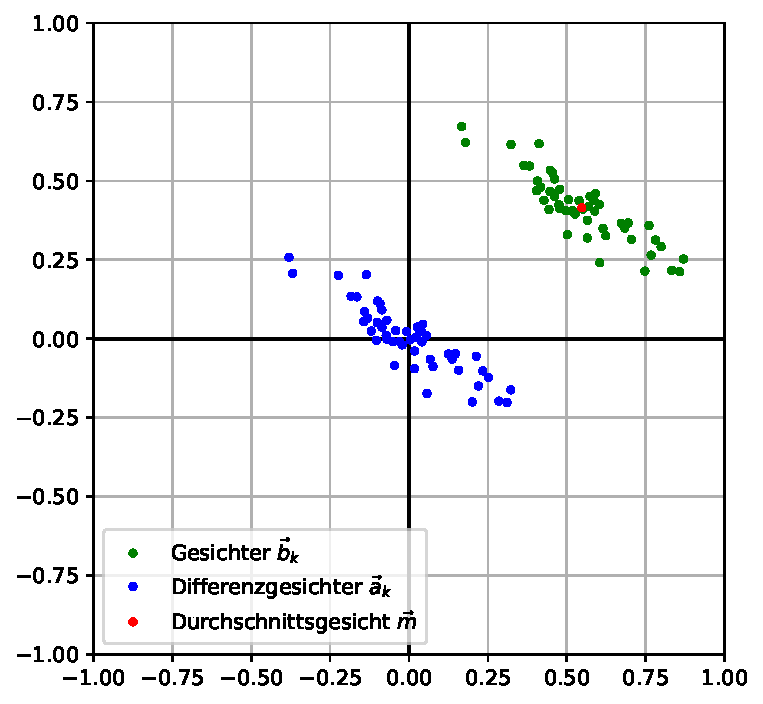
\includegraphics[width=0.5\textwidth]{images/facespace/meandiff}
	\caption{Die Gesichter werden um den Ursprung zentriert indem man das Durchschnittsgesicht subtrahiert.}
	\label{fig:meandiff}
\end{figure}
\begin{aufgabe} \label{aufg:hmmc}
	Nennen Sie einen Unterschied und eine Gemeinsamkeit der vereinfachten Darstellung links in Abbildung~\ref{fig:meandiff} zu unserer tatsächlichen Situation mit Bildern von Gesichtern.
	Gehen Sie davon aus, dass unsere Bilder eine Auflösung von $M=180$ und $N=144$ haben, wie im letzten Kapitel.
\end{aufgabe}
\begin{losung*}
	Als Vektoren aufgefasst sind die Gesichter Punkte im $\mathbb R^{M\cdot N}$.
	Für $M=180$ und $N=144$ wären das Punkte im $\mathbb R^{25'920}$ und nicht im $\mathbb R^2$ wie in der Abbildung.
	Anders ausgedrückt zeigt die Abbildung den Spezialfall $M\cdot N=2$.
	Das entspricht Bilder die nur aus zwei Pixeln bestehen.
	Andererseits wird in der Abbildung korrekt gezeigt, dass die Komponenten der Gesichts-Vektoren $\vec b_k$ nur Werte zwischen 0 und 1 annehmen.
	Zudem sind die Differenzgesichter richtigerweise genau als Verschiebung der Gesichts-Vektoren um $-\vec m$ dargestellt.
\end{losung*}
Die Eigengesichter werden nun aus den Differenzgesichtern konstruiert.
Dies wird im nächsten Kapitel behandelt.